\begin{dbltab}
   \begin{center}
\footnotesize\begin{tabular}{ | l || c | c | c | c | c | c | c | c | c | c |}
\hline
\multirow{2}{*}{\textbf{Program}} & \multicolumn{5}{c |}{\textbf{Queue
   Operations}} & \multicolumn{5}{c |}{\textbf{Facts Derived}} \\ \cline{2-11}
& 1 & 2 & 4 & 8 & 16 & 1 & 2 & 4 & 8 & 16\\ \hline
\hline
SSSP - Regular & 199.1K & 203.1K & 202.7K & 203.8K & 206.4K & 3.3M & 3.0M & 3.4M & 3.5M & 3.3M \\
SSSP - Coordinated & 959.0K & 924.3K & 891.0K & 966.3K & 1.0M & 2.0M & 2.3M & 2.3M & 2.2M & 2.3M \\
SSSP - Buffered & 1.0M & 1.0M & 1.1M & 1.0M & 1.1M & 2.0M & 2.1M & 2.3M & 2.3M & 2.4M \\
\hline
HT - Regular & 25.6M & 33.3M & 34.8M & 36.1M & 34.8M & 235.7M & 298.3M & 312.1M & 317.5M & 310.3M \\
HT - Coordinated & 51.6M & 55.2M & 85.9M & 79.9M & 75.6M & 129.2M & 183.4M & 254.1M & 242.0M & 252.4M \\
HT - Local-Only & 51.6M & 54.9M & 81.0M & 76.7M & 67.3M & 129.2M & 180.8M & 221.5M & 217.6M & 207.4M \\
\hline
LBP - Regular & 15.7M & 17.8M & 16.0M & 11.3M & 8.5M & 160.2M & 171.0M & 149.9M & 107.5M & 85.1M \\
SBP - Coordinated & 97.2M & 97.4M & 90.0M & 84.3M & 79.2M & 76.8M & 80.7M & 79.2M & 79.0M & 79.3M \\
\hline \hline
MiniMax - Regular & 16.4M & 18.3M & 20.5M & 19.4M & 20.9M & 76.4M & 76.4M & 76.4M & 76.4M & 76.4M \\
MiniMax - Coordinated & 52.0M & 52.0M & 52.0M & 52.0M & 52.0M & 76.4M & 76.4M & 76.4M & 76.4M & 76.4M \\
\hline
N Queens - Regular & 8.4K & 14.4K & 17.7K & 16.6K & 19.3K & 167.1M & 167.1M & 167.1M & 167.1M & 167.1M \\
N Queens - Coordinated & 57.1M & 24.7M & 1.1M & 141.1K & 41.6K & 167.1M & 167.1M & 167.1M & 167.1M & 167.1M \\
N Queens - Static & 57.1M & 47.2M & 3.4M & 1.5M & 209.2K & 167.1M & 167.1M & 167.1M & 167.1M & 167.1M \\
\hline
\end{tabular}
\vspace*{.5ex}
\end{center}
\scap{queue_instructions}{Total number of queue operations and facts derived per program. An
   operation to a regular queue counts as 1 instruction, while an operation to
   a priority queue costs the number of
   \emph{percolate-up}/\emph{percolate-down} steps performed.}
\end{dbltab}

Coordination introduces overhead in two major ways.  First, in
manipulating the priority queues which require operations on a min
heap.  Second, in potentially requiring more lock operations as we
move nodes between queues and within the priority queue.  As we show
next, this overhead is minimal and is compensated by the resulting improved schedules
and memory locality that more than make up for the overhead.

As can be seen in Table~\ref{queue_instructions} all the coordinated
versions of the programs require significantly more queue operations.
The data for this table comes from recording the number of queue
operations and facts derived.  Queue operations represent the number
of normal queue operations executed (each costs 1) plus the number of
\emph{percolate-up}/\emph{percolate-down} operations executed for each
manipulation of the priority queue.  As expected, programs which rely
on prioritizing the order of execution to obtain better asymptotic
complexity (e.g., SSSP), improve in overall running time at the cost of
more queue operations.  In all cases, coordination adds a significant
number of total queue operations, but the resulting overhead is more
than compensated for by an improved schedule and reduction in number
of facts produced. For MiniMax and N Queens, the number of facts
derived is the same for all configurations, as expected. The
performance seen for those programs arise from reduced memory usage
and improved memory locality.

An interesting artifact of effectively parallelizing the code is that
the priority queue on each thread is smaller, so the total number of
priority queue operations is significantly reduced as the depth of the
min heap on each thread is reduced.  This is particularly evident for
the N Queens program.

\begin{topfig}
   \begin{center}
      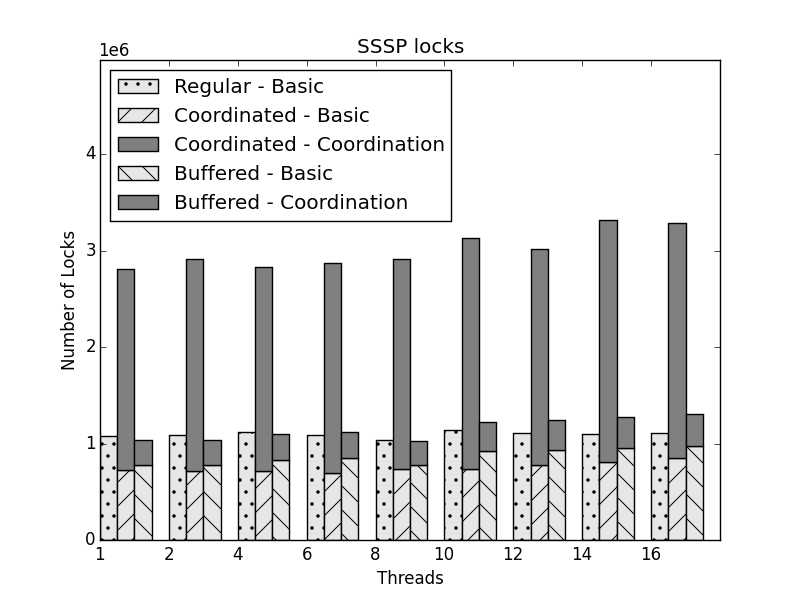
\includegraphics[width=6.5cm]{results/locks/sssp-locks.png}
   \end{center}
  \scap{locks:SSSP}{Locking statistics for SSSP.
     \mytt{Coordinated} refers to the program in
     Fig.~\ref{results:sssp_uspowergrid}, while \mytt{Buffered} is a more
     optimized version of the same program where coordination operations are
     buffered before application.}
\end{topfig}

\begin{topfig}
   \begin{center}
      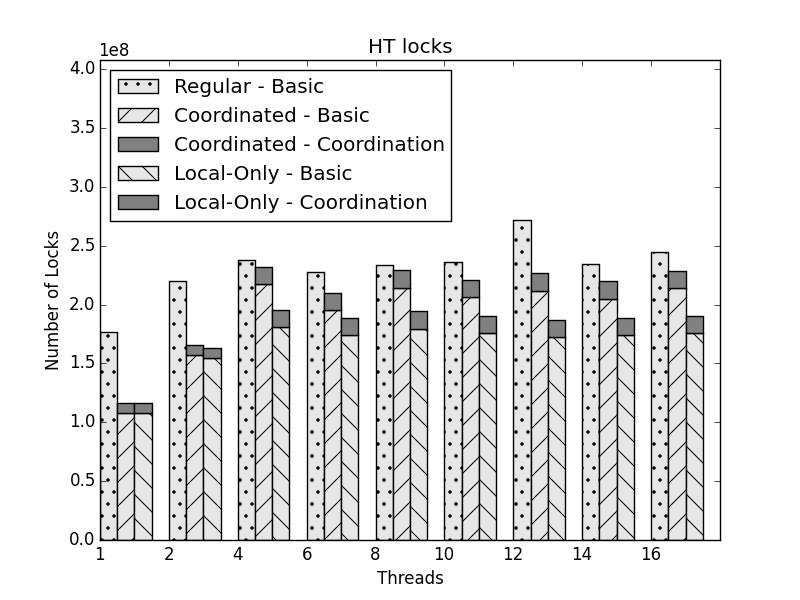
\includegraphics[width=6.5cm]{results/locks/ht-locks.png}
   \end{center}
  \scap{locks:HT}{Locking statistics for HT. Coordination reduces
     the overall number of locks used, while further optimization for locality
     reduces the locks even further.}
\end{topfig}

We next investigate the effect of coordination on the synchronization
overhead that comes from the use of more locks.  We measured the
\emph{basic locks}, the number of locks acquired
in the original LM virtual machine and \emph{coordination locks}, the
number of locks acquired to perform coordination operations.  We also
measured how often \mytt{lock()} operations fail to acquire
the lock on the first attempt.  Lock failures happen so infrequently
(less than 1\% of the time) that they cannot be seen on the figures.

Fig.~\ref{results:sssp_uspowergrid} shows the number of locks acquired
for the SSSP program.  The first bar in each group shows the number of
locks acquired for the regular version of the program.  The
second bar shows the basic and coordination locks acquired for the coordinated
version of SSSP when every newly derived fact and priority operation is carried out
immediately.  This leads to a significant increase in total locks
acquired often because the priority of a node is changed many times
before it is operated on.  The third bar shows the effect of buffering
priority operations before applying them.  This significantly reduces
the lock overhead, but as can be seen in
Table~\ref{queue_instructions}, increases the number of queue operations
slightly.  This slight increase comes from the fact that buffering
delays the change in priorities and some longer paths can sometimes be
investigated unnecessarily.

Fig.~\ref{locks:HT} shows the locking behavior of the heat transfer
program.  The behavior is representative of the other programs. In general, there
is a drop in the total number of locks acquired and coordination locks
represent a small fraction of the total number of locks acquired. \textbf{Local-Only}
further reduces locking by keeping more derivations local to a thread.

Overall, the additional overhead introduced by supporting coordination
is more than offset by improved schedules and increased locality.
While there are more locks to manage the total cost of lock operations,
the numbers do not change significantly (and is often reduced) when coordination
is added.  And, although the priority coordination significantly
increases the cost of queueing it is offset by reducing the number of
total facts derived.
